% ---- ETD Document Class and Useful Packages ---- %
\documentclass{ucetd}
\usepackage{subfigure,epsfig,amsfonts}
\usepackage{natbib}
\usepackage{amsmath}
\usepackage{amssymb}
\usepackage{amsthm}
\usepackage[toc,page]{appendix}
\usepackage[labelfont=bf]{caption}
\usepackage{rotating}
\usepackage[dvipsnames]{xcolor}
\usepackage{url}
\usepackage{bm}

%% Use these commands to set biographic information for the title page:
\title{The statistical mechanics of transcriptional control}
\author{Clayton W. Seitz}
\department{Department of Physics}
\division{Physical Sciences}
\degree{Doctor of Philosophy}
\date{Spring 20XX}

%% Use these commands to set a dedication and epigraph text

\epigraph{Epigraph}



\begin{document}
%% Basic setup commands
% If you don't want a title page comment out the next line and uncomment the line after it:
\maketitle
%\omittitle

% These lines can be commented out to disable the copyright/dedication/epigraph pages
\makecopyright
%\makededication


%% Make the various tables of contents
\tableofcontents
%\listoffigures
%\listoftables

%\acknowledgments
% Enter Acknowledgements here

\abstract

Eukaryotic transcription is episodic, consisting of a series of transcriptional bursts, Bursty transcriptional dynamics are well-exemplified by the transient expression of pro-inflammatory guanylate binding proteins (GBPs) - a group interferon-inducible GTPases that restrict the replication of intracellular pathogens [XXX]. Classical models of gene regulation explain transcriptional bursts by invoking stochastic binding and unbinding of transcription factors, RNA polymerase and mediator proteins at enhancer or promoter sequences. However, more recent studies have pointed towards a more cooperative picture of transcriptional control where phase-separated aggregates of DNA, RNA, and proteins form higher-order structures to control gene expression. For example, both chromatin immunoprecipitation and super resolution imaging have captured the phase separation of super-enhancer-binding proteins MED1 and BRD4 in transcriptional condensates at the \textit{Essrb} genomic locus [XXX]. Furthermore, fluorescence microscopy techniques have colocalized MED1 and BRD4 with the GBP gene cluster alongside a reduction in the degree of disorder of 3D chromatin structure in murine macrophages after infection with \textit{Mycobacterium tuberculosis}. Taken together, these results suggest that phase separation may play a role in the reorganization of chromatin structure during trancriptional control of innate immune response genes [XXX]. Here, we hypothesize that phase separation reduces the entropy of chromatin structure in order to induce bursty gene expression. Using single molecule localization microscopy (SMLM) to obtain super-resolution images of the H2B protein, we intend to demonstrate simultaneous (i) loss of disorder in chromatin structure (ii) formation of transcriptional condensates containing MED1 and BRD4 and (iii) non-Poissonian gene expression. The following sections discuss recent the biological evidence in more detail and summarize the single molecule microscopy techniques and biophysical models we employ to study the interactions between transcriptional condensates and the chromatin scaffold.

\clearpage

\mainmatter

\chapter{Single molecule localization microscopy}


\section{Stochastic optical reconstruction microscopy}

\section{PSF engineering in single molecule localization microscopy}

Born and Wolf's approximation, Lateral and axial point spread functions, Potentially double helix point spread functions for 3D storm

\subsection{Fisher information theory for parameter estimation in single molecule microscopy}

\section{Bounding parameter uncertainty in single molecule localization}

\subsection{Point spread functions in widefield microscopy}

Most detectors used for imaging have many elements (pixels) so that we can record an image projected onto the detector by a system of lenses. In fluorescence imaging, this is usually a relay consisting of an objective lens and a tube lens to focus the image onto the camera. Due to diffraction, any point emitter, such as a single fluorescent molecule, will be registered as a diffraction limited spot. The profile of that spot is often described as a Gaussian point spread function (Richardson and Wolf)

\begin{equation}
\mathrm{PSF}(x,y) = \frac{1}{2\pi\sigma^{2}}\exp\left(-\frac{(x-x_{0})^{2}+(y-y_{0})^{2}}{2\sigma^{2}}\right)
\end{equation}

where $(x_0,y_0)$ defines the coordinates of a single fluorescent molecule on a detector $\mathcal{D}$. 

\begin{figure}[t!]
\centering
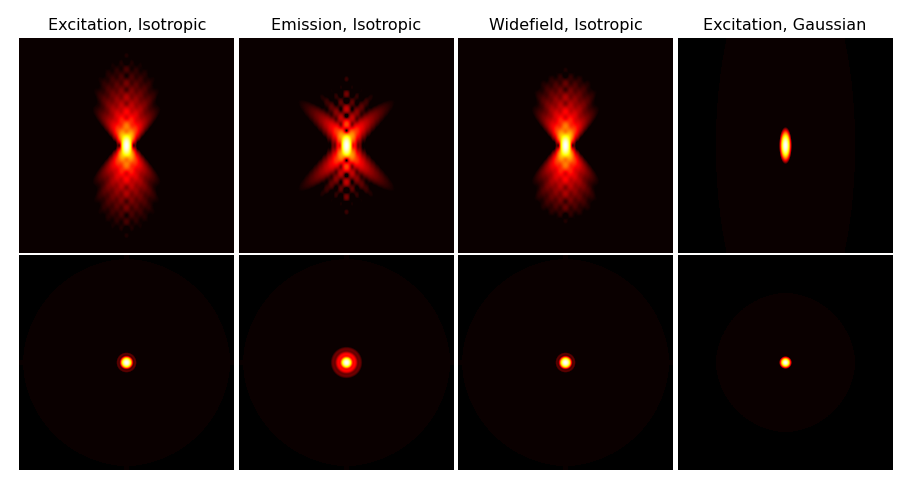
\includegraphics[width=150mm]{psf-1}
\caption{Cartoon of a excitatory-inhibitory neural network receving a time-dependent feedforward current $F(t)$, feedback current $R(t)$, and synaptic noise $\xi(t)$. Excitatory neurons are shown in red and inhibitory neurons shown in blue. Synaptic current is drawn to be instantaneous and syanptic weights $J_{ij}$ are not functions of time. Feedforward inputs could be weighted Poisson processes where $F$ defines the rates, for example.}
\end{figure}

\begin{figure}[t!]
\centering
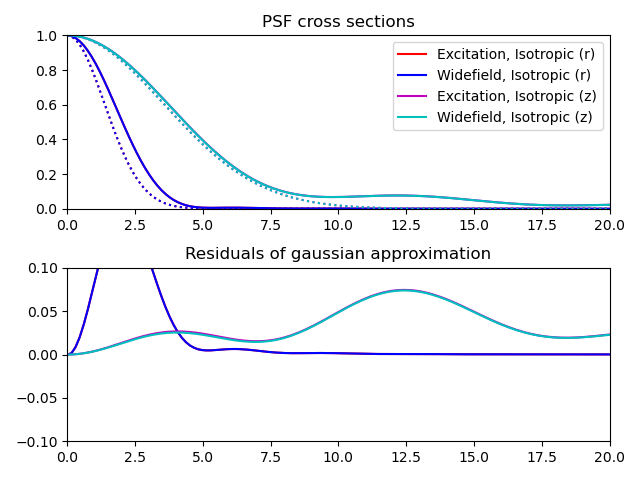
\includegraphics[width=150mm]{psf-2}
\caption{Cartoon of a excitatory-inhibitory neural network receving a time-dependent feedforward current $F(t)$, feedback current $R(t)$, and synaptic noise $\xi(t)$. Excitatory neurons are shown in red and inhibitory neurons shown in blue. Synaptic current is drawn to be instantaneous and syanptic weights $J_{ij}$ are not functions of time. Feedforward inputs could be weighted Poisson processes where $F$ defines the rates, for example.}
\end{figure}


\subsection{Maximum a posteriori estimation of PSF parameters}

Maximum a posteriori estimation of parameters

\begin{align*}
\theta^{*}_{\mathrm{MAP}} &= \underset{\theta}{\mathrm{argmax}} \;P(\theta|\mathcal{X})\\
&= \underset{\theta}{\mathrm{argmax}} \;\frac{\mathcal{L}_{\theta}\pi(\theta)}{\int_{\theta}\mathcal{L}_{\theta}\pi(\theta)}
\end{align*}


where $\mathcal{L}_{\theta} = \mathcal{L}(\theta|\mathcal{X})$ is the likelihood function and $\pi(\theta)$ a prior on the parameters. Furthermore, we will assume that $\pi(\theta)$ is a uniform distribution. An image captured by a camera can be loosely thought of as histogram of photon arrivals and a discretized form of the density $\mathrm{PSF}(x,y)$ over an integration time $\tau$. If $\mathrm{PSF}(x,y)$ can be approximated as constant in time ($\tau << 1$), the value at a pixel approaches an integral of this density over the pixel:

\begin{equation}
\lambda_{k} = \gamma\cdot\int_{\mathcal{D}_{k}} q(x,y)dxdy
\end{equation}

Put another way, the variable $\lambda_{k}$ at a pixel $k$ defines the probability of observing a photon per unit time and therefore we can define the number of photons arriving at each pixel as a random variable

\begin{equation*}
P(S_{k}) = \mathrm{Poisson}(\lambda_{k})
\end{equation*}


It would be convenient to obtain an analytical expression for $\lambda_{k}$ given the parameters of the point spread function $\theta = (x_0,y_0,\sigma)$. This can be done by making use of the error function

\begin{equation*}
\mathrm{erf}(x) \equiv \frac{2}{\sqrt{\pi}}\int_{0}^{x} \exp(-t^{2})dx
\end{equation*}

where $t = \frac{x}{\sqrt{2}\sigma}$. We just need to rescale this so it is appropriate for a standard normal distribution. We need something like

\begin{equation*}
F(x) = \frac{1}{\sqrt{2\pi}}\int_{0}^{x} \exp(-t^{2})dx
\end{equation*}

so we rescale the error function by $\beta = 1/2\sqrt{2}$. Of course, this can also be used to construct the integral over an arbitrary interval $[a,b]$

\begin{equation*}
\mathrm{erf}(b) - \mathrm{erf}(a) = \frac{2\beta}{\sqrt{\pi}}\int_{\frac{a}{\sqrt{2}\sigma}}^{\frac{b}{\sqrt{2}\sigma}} \exp(-t^{2})dt
\end{equation*}

We use this result to compute the Poisson rate $\lambda_{k}$ at pixel $k$. Now, the Poisso rate is in general given by

\begin{align*}
\lambda_{k} &= \frac{1}{2\pi}\left(\int_{x_{k}}^{x_{k+1}}\exp\left(-\frac{(x-x_{0})^{2}}{2\sigma^{2}}\right)dx\right)\left(\int_{y_{k}}^{y_{k+1}}\exp\left(-\frac{(y-y_{0})^{2}}{2\sigma^{2}}\right)dy\right)\\
\end{align*}

Let $t = (x-x_{0})/\sqrt{2}\sigma$ and $z = (y-y_{0})/\sqrt{2}\sigma$ and write constant in terms of $\beta$

\begin{align*}
\lambda_{k} &= \frac{4\beta^{2}}{\pi}\left(\int_{t_{k}}^{t_{k+1}}\exp\left(-t^{2}\right)dx\right)\left(\int_{z_{k}}^{z_{k+1}}\exp\left(-z^{2}\right)dy\right)\\
&= \beta^{2}\left[\mathrm{erf}(t_{k+1}) - \mathrm{erf}(t_{k})\right]\left[(\mathrm{erf}(z_{k+1}) - \mathrm{erf}(z_{k})\right]
\end{align*}

where for example $t_{k} = (x_{k}-x_{0})/\sqrt{2}\sigma$


Detectors often suffer from dark noise (thermal noise) and there may also be a background signal. Considering the former first, we define another r.v. $W_{k}$ which represents Gaussian dark noise associated with pixel $k$. Unless otherwise specified we will always assume that $W_{k} \sim \mathcal{N}(m_{k},\sigma_{w,k}^{2})$. We represent our corrupted signal as another random variable $H_{k}$. As a side note, we define $S_{k}$ to have units of photons $[\mathrm{p}]$, while $H_{k}$ has units of photoelectrons $[e^{-}]$. The conversion factor between the two is the gain of the detector element $g_{k}\; [e^{-}\mathrm{p}^{-1}]$.

Dropping the pixel subscripts for the moment, the Fourier transform of a normal distribution $\mathcal{N}(\mu,\sigma_{w}^{2})$, or its characteristic function reads

\begin{align*}
\tilde{P}(W) &= \int_{-\infty}^{\infty} \frac{1}{\sqrt{2\pi}\sigma_{w}}e^{-\frac{(x-\mu)^{2}}{2\sigma_{w}^{2}}}e^{-i\omega x} dx\\
&= \frac{e^{-\frac{\sigma_{w} ^2 \omega ^2}{2}+i \mu  \omega }}{\sqrt{2 \pi } }
\end{align*}

On the other hand for $\lambda >> 1$ we can approximate the Poisson distribution as a normal distribution $\mathcal{N}(\lambda, \sqrt{\lambda})$ on countable support. We can then then write the likelihood function $\mathcal{L}_{\theta,k}$ as the inverse Fourier transform of the product of these two characteristic functions

\begin{align*}
\mathcal{L}_{\theta,k} &= \frac{1}{\sqrt{2\pi}}\int_{-\infty}^{\infty} e^{-\frac{\sigma_{k} ^2 \omega ^2}{2}+i \mu_{k}  \omega } e^{-\frac{\lambda_{k} \omega ^2}{2}+i \lambda_{k}  \omega }  e^{-i\omega x} d\omega\\
&= \frac{1}{\sqrt{2\pi(\lambda_{k} + \mu_{k}^{2})}}e^{-\frac{(-x+\mu_{k}+\lambda_{k})^{2}}{2(\lambda_{k}+\mu_{k}^{2})}}
\end{align*}

We can now return to the original optimization problem 

\begin{align*}
\theta^{*}_{\mathrm{MAP}} &= \underset{\theta}{\mathrm{argmax}} \;\ \pi(\theta)\mathcal{L}_{\theta}\\
&= \underset{\theta}{\mathrm{argmax}} \; \prod_{k}\mathcal{L}_{\theta,k}\\
&= \underset{\theta}{\mathrm{argmax}} \; \sum_{k}\log \mathcal{L}_{\theta,k}
\end{align*}

\begin{align*}
\sum_{k}\log \mathcal{L}_{\theta,k} = \sum_{k}-\frac{(-x+\mu_{k}+\lambda_{k})^{2}}{2(\lambda_{k}+\mu_{k}^{2})} -\log\left(\sqrt{2\pi(\lambda_{k} + \mu_{k}^{2})}\right)
\end{align*}

Maximizing $\mathcal{L}_{\theta}$ is therefore equivalent to maximizing $\mathcal{L}_{\theta,k}$ at every pixel. Taking the derivative of the first term with respect to a parameter $\theta$

\begin{align*}
&\frac{\partial}{\partial \theta} \left(\frac{(-x+\mu_{k}+\lambda_{k})^{2}}{2(\lambda_{k}+\mu_{k}^{2})} \right)\\
&= \left(\frac{4(\lambda_{k}+\mu_{k}^{2})(-x+\mu_{k}+\lambda_{k})\frac{\partial \lambda_{k}}{\partial \theta} - 2\frac{\partial \lambda_{k}}{\partial \theta} (-x+\mu_{k}+\lambda_{k})^{2}}{4(\lambda_{k}+\mu_{k}^{2})^{2}} \right)
\end{align*}

\begin{align*}
\frac{\partial}{\partial \theta} \log\left(\sqrt{2\pi(\lambda_{k} + \mu_{k}^{2})}\right) &= \frac{1}{2(\lambda_{k} + \mu_{k}^{2})}\frac{\partial \lambda_{k}}{\partial \theta}
\end{align*}

\begin{align*}
\frac{\partial \lambda_{k}}{\partial x_{0}} &= \beta^{2}\left(\int_{x_{k}}^{x_{k+1}}\frac{\partial}{\partial x_{0}}\exp\left(-\frac{(x-x_{0})^{2}}{2\sigma^{2}}\right)dx\right)\left[(\mathrm{erf}(z_{k+1}) - \mathrm{erf}(z_{k})\right]\\
&= \frac{\beta^{2}}{\sigma^{2}}\left(\int_{x_{k}}^{x_{k+1}} (x-x_{0})\exp\left(-\frac{(x-x_{0})^{2}}{2\sigma^{2}}\right)dx\right)\left[(\mathrm{erf}(z_{k+1}) - \mathrm{erf}(z_{k})\right]
\end{align*}

\begin{align*}
\int_{x_{k}}^{x_{k+1}} x\exp\left(-\frac{(x-x_{0})^{2}}{2\sigma^{2}}\right)dx - x_{0}\int_{x_{k}}^{x_{k+1}} \exp\left(-\frac{(x-x_{0})^{2}}{2\sigma^{2}}\right)dx
\end{align*}

\begin{align*}
\int_{x_{k}}^{x_{k+1}} x\exp\left(-\frac{(x-x_{0})^{2}}{2\sigma^{2}}\right)dx &= \sigma\sqrt{2\pi}\;\bigg|_{x_{k}}^{x_{k+1}}x  - \int_{x_{k}}^{x_{k+1}} \exp\left(-\frac{(x-x_{0})^{2}}{2\sigma^{2}}\right)dx\\
&= \sqrt{2\pi}\sigma\Delta - \mathrm{erf}(t_{k+1}) - \mathrm{erf}(t_{k})
\end{align*}


\subsection{Fisher information and the Cramer-Rao bound}

Suppose we are given samples from a normal distribution with unknown parameters. We then decide to build a model normal distribution. Perhaps we define a likelihood function over the $\mu-\sigma$ plane based on a set of samples, does the likelihood of the data vary? If the likelihood surface is flat, all parameter sets would be equally likely and the data does not appear to carry much information about the parameters. If the surface has a number of bumps or inflection points, then we expect our data does carry information about the parameters. This ``bumpiness" of the likelihood surface is measured by computing the variance the second derivative of the likelihood over the parameter space\\

\vspace{0.2in}
The log-likelihood of an image under parameters $\theta = (x_{0},y_{0},\sigma^{2},\sigma_{w}^{2},g_{k})$, assuming each pixel is an independent but not identical random variable, reads

\begin{align*}
\ell(H|\theta) = \log\prod_{k}^{M^{2}} P(H_{k}|\theta) = \sum_{k=1}^{M^{2}} \ell (H_{k}|\theta)
\end{align*}


When there are many parameters, the Fisher Information (second moment of the score) is a matrix

\begin{align*}
I_{ij}(\theta) &= \underset{\theta}{\mathbb{E}}\left[\frac{\partial}{\partial\theta_{i}} \left(\ell(H|\theta)\right)\frac{\partial}{\partial\theta_{j}} \left(\ell(H|\theta)\right)\right]\\
\end{align*}

The only elements of the matrix of interest are on the diagonal, which allows us to write

\begin{align*}
I(\theta_{i}) &= \underset{\theta}{\mathbb{E}}\left[\sum_{k}\frac{\partial^{2}}{\partial\theta_{i}^{2}}  \ell (H_{k}|\theta)\right]\\
\end{align*}

At this point, we need to evaluate the second derivative w.r.t each of the parameters in $\theta = (x_{0},y_{0},\sigma^{2})$. We have shown that the model for the number of photoelectrons at a pixel is


\chapter{Statistical mechanics of gene regulation}

\section{Introduction}

\section{Transcriptional bursts and chromatin architecture}

\section{Transcriptional condensates: a phase separation model for transcriptional control}

Heavily influenced by Young's group at MIT


\section{Brief introduction to polymer dynamics}

\section{Statistical mechanics of transcriptional condensates}

\section{The chemical master equation and finite state projection}

The central assumption underlying a Markov process, is the memoryless property

\begin{equation*}
P(X_{t}|X_{t-1}, X_{t-2}, ..., X_{t-N}) = P(X_{t}|X_{t-1})
\end{equation*}

A single Markov chain is the set of states $\bm{X} = \{X_{1},X_{2},...,X_{N}\}$. Such a set can be generated provided that $P(X_{t}|X_{t-1})$ is known. To capture $P(X_{t}|X_{t-1})$ for all possible pairs $X_{t}$ and $X_{t-1}$, we define a square transition matrix $T\in \mathcal{R}^{N\times N}$ where $N = |\Omega|$. As such, the elements of $T$ represent the probability of a transition from a state $\omega_{j}$ to $\omega_{i}$ in a unit time

\begin{equation*}
T_{ij} = \mathrm{Pr}\left(X_{t}=\omega_{i}, | \;X_{t-1}=\omega_{j}\right)
\end{equation*}

Under these definitions, the row $T_{i}$ represents the present time, and is a conditional  probability distribution $P(\omega | X_{t-1} = \omega_{j})$ which requires that

\begin{equation*}
\sum_{j}T_{ij} = \sum_{j} P(X_{t} = \omega_{j} | X_{t-1} = \omega_{i}) = 1
\end{equation*}

The matrix $T$ is not necessarily symmetric $T_{ij} \neq T_{ji}$. One should note that the columns $T_{j}$ \emph{do not} define a probability distribution $P(X_{t} = \omega_{i} | X_{t-1} = \omega_{j})$ and therefore do not necessarily sum to unity. The probability $P(X_{t} = \omega_{i} | X_{t-1} = \omega_{j})$ has no meaning in this context, since we have defined the rows to represent a probability of the future given the present. We simply sample $X_{t} \sim P(X_{t} = \omega_{j} | X_{t-1} = \omega_{i})$, assign $i=j$, and repeat. It directly follows from the fundamental rules of probability, the first order dynamics for a \textbf{particular} state $\omega_{i}$: $P(\omega_{i},t)$ is given by

\begin{equation}
P(\omega_{i},t+dt) = P(\omega_{i},t) + \mathcal{J}_{i}dt
\end{equation}

The net probability current $\mathcal{J}_{i}$ must be 

\begin{equation*}
\mathcal{J}_{i} = \sum_{i}T_{ij}P(\omega_{j},t) - \sum_{j}T_{ij}P(\omega_{i},t)\\
\end{equation*}

The first is a sum on a column and the second a sum on a row. This can be simplified further by noticing that the normalization condition implies

\begin{align*}
T_{ij} &= 1 - \sum_{j}T_{ij}(1-\delta_{ij})\\
&= 1 - \sum_{j}T_{ij} + \sum_{j}T_{ij}\delta_{ij}
\end{align*}


\begin{align*}
\mathcal{J}_{i} &= \sum_{i}T_{ij}P(\omega_{j},t) - \sum_{j}T_{ij}P(\omega_{i},t)\\
&= \sum_{i}\left(1 - \sum_{j}T_{ij} + \sum_{j}T_{ij}\delta_{ij}\right)P(\omega_{j},t) - \sum_{j}T_{ij}P(\omega_{i},t)\\
&= |\Omega| - |\Omega| + \sum_{i}\sum_{j}T_{ij}P(\omega_{j},t)\delta_{ij} - \sum_{j}T_{ij}P(\omega_{i},t)\\
&= \sum_{j}T_{ji}P(\omega_{j},t) - T_{ij}P(\omega_{i},t)\\
\end{align*}

Notice that the Kronecker delta effectively just swaps the index. Taking the limit of (1.1), we arrive at the \textbf{master equation}


\begin{equation*}
\frac{\partial P(\omega_{i})}{\partial t} = \sum_{j}T_{ji}P(\omega_{j},t) - T_{ij}P(\omega_{i},t)
\end{equation*}

It is common to then define an operator $\bm{W}$ s.t. $W_{ij} = T_{ij}$ and $W_{ii} = -\sum_{j}T_{ij}$ 

\begin{align*}
\frac{dP(\omega_{i})}{dt} = \sum_{j}W_{ij}P(\omega_{j}) \rightarrow \frac{dP(\bm{\omega})}{dt} = \mathcal{J}(\bm{\omega}) = \mathbf{W}P(\bm{\omega})
\end{align*}

This operator form has a solution in terms of a matrix exponential

\begin{equation*}
P(\bm{\omega}, t) = \exp(\mathcal{J}(\bm{\omega}))
\end{equation*}

This matrix exponential is intractable for large $|\Omega|$. However, in the Finite State Projection algorithm, it is possible to truncate the state space $\Omega \rightarrow \tilde{\Omega}$ and obtain good estimates $\tilde{P}(\bm{\omega}, t)$ with some certificate of accuracy.

\subsection{Sequential tempered Markov Chain Monte Carlo}




\begin{appendices}
\chapter{Derivation of the Fokker Planck Equation}

\subsection{Kramers-Moyal Expansion}

Gixen many instantiations of a stochastic xariable $x$, we can construct a normalize histogram oxer all obserxations as a function of time $P(x,t)$. Howexer, in order to systematically explore the relationship between the parameterization of the process and $P(x,t)$ we require an expression for $\dot{P}(x,t)$. If we make a fundamental assumption that the exolution of $P(x,t)$ follows a Markox process i.e. its exolution has the memoryless property, then we can write

\begin{equation}
P(x', t) = \int T(x', t | x, t-\tau)P(x, t-\tau)dx
\end{equation} 

which is known at the Chapman-Kolmogorox equation. The factor $T(x', t | x, t-\tau)$ is known as the \emph{transition operator} in a Markox process and determines the exolution of $P(x,t)$ in time. We proceed by writing $T(x', t | x, t-\tau)$ in a form referred to as the Kramers-Moyal expansion

\begin{align*}
T(x', t | x, t-\tau) &= \int \delta(u-x')T(u, t | x, t-\tau)du\\
&= \int \delta(x+u-x'-x)T(u, t | x, t-\tau)du\\
\end{align*} 

If we use the Taylor expansion of the $\delta$-function 

\begin{equation*}
\delta(x+u-x'-x) = \sum_{n=0}^{\infty} \frac{(u-x)^{n}}{n!}\left(-\frac{\partial}{\partial x}\right)^{n}\delta(x-x')
\end{equation*}

Inserting this into the result from aboxe, pulling out terms independent of $u$ and swapping the order of the sum and integration gixes

\begin{align}
T(x', t | x, t-\tau) &= \sum_{n=0}^{\infty} \frac{1}{n!}\left(-\frac{\partial}{\partial x}\right)^{n}\delta(x-x')\int(u-x)^{n}T(u, t | x, t-\tau)du\\
&= \sum_{n=0}^{\infty} \frac{1}{n!}\left(-\frac{\partial}{\partial x}\right)^{n}\delta(x-x')M_{n}(x,t)
\end{align} 

noticing that $M_{n}(x,t) = \int(u-x)^{n}T(u, t | x, t-\tau)du$ is just the $n$th moment of the transition operator $T$. Plugging (2.6) back in to (2.4) gixes 

\begin{align}
P(x, t) &= \int \left(1 + \sum_{n=1}^{\infty} \frac{1}{n!}\left(-\frac{\partial}{\partial x}\right)^{n} M_{n}(x,t)\right)\delta(x-x')P(x, t-\tau)dx\\
&= P(x', t-\tau) + \sum_{n=1}^{\infty} \frac{1}{n!}\left(-\frac{\partial}{\partial x}\right)^{n} \left[M_{n}(x,t)P(x,t)\right]
\end{align} 

Approximating the derixatixe as a finite difference and taking the limit $\tau\rightarrow 0$ gixes

\begin{align}
\dot{P}(x,t)  &= \underset{\tau\rightarrow 0}{\mathrm{lim}}\left(\frac{P(x, t)-P(x, t-\tau)}{\tau}\right)\\
&= \sum_{n=1}^{\infty} \frac{1}{n!}\left(-\frac{\partial}{\partial x}\right)^{n} \left[M_{n}(x,t)P(x,t)\right]
\end{align} 

which is formally known as the Kramers-Moyal (KM) expansion. The Fokker-Planck equation is a special case of (2.10) where we neglect terms $n>2$ in the \emph{diffusion approximation}.


Consider the following Ito stochastic differential equation 

\begin{align*}
d\vec{x} = F(\vec{x},t) + G(\vec{x},t)dW
\end{align*}

The SDE gixen aboxe corresponds to the Kramers-Moyal expansion (KME) of a transition density $T(x',t'|x,t)$ see (Risken 1989) for a full derixation.

\begin{align}
\frac{\partial P(x,t)}{\partial t}  &= \sum_{n=1}^{\infty} \frac{1}{n!}\left(-\frac{\partial}{\partial x}\right)^{n} \left[M_{n}(x,t)P(x,t)\right]
\end{align}

where $M_{n}$ is the $n$th moment of the transition density. In the diffusion approximation, the KME becomes the Fokker-Planck equation (FPE) (Risken 1989). For the sake of demonstration, consider the univariate case with random variable $x$ and the form of $T(x',t'|x,t)$ is a Gaussian with mean $\mu(t)$ and variance $\sigma^{2}(t)$. In this scenario, the FPE applies because $M_{n} = 0$ for all $n > 2$. Given that the drift $M_{1}(x,t) = \mu(t)$ and the diffusion $M_{2}(x,t) = \sigma^{2}(t)$, the FPE reads

\begin{align}
\frac{\partial P(x,t)}{\partial t}  &= \left(-\frac{\partial}{\partial x}M^{(1)}(t) + \frac{1}{2}\frac{\partial^{2}}{\partial x^{2}}M^{(2)}(t)\right)P(x,t)
\end{align}

We can additionally define the term in parentheses as a differential operator acting on $P(x,t)$

\begin{align}
\hat{\mathcal{L}}_{FP} = \left(-\frac{\partial}{\partial x}M^{(1)}(t) + \frac{1}{2}\frac{\partial^{2}}{\partial x^{2}}M^{(2)}(t)\right)
\end{align}

It is common to additionally define the probability current $J(x,t)$ as 

\begin{align}
J(x,t)  &= \left(M^{(1)}(t) - \frac{1}{2}\frac{\partial}{\partial x}M^{(2)}(t)\right)P(x,t)
\end{align}

This definition provides some useful intuition. The value of $J(x,t)$ is the net probability flux into the interval between $x$ and $x+dx$ at at time $t$. This also allows us to write the FPE as a continuity equation

\begin{align}
\frac{\partial P(x,t)}{\partial t} = -\frac{\partial J(x,t)}{\partial x}
\end{align}
\end{appendices}



\section{Poisson processes}

The Poisson process can be derived very quickly by noticing that it is simply the continuous-time limit of the Binomial distribution.

\begin{align*}
B(m;t) &= {n\choose m}\lambda^{m}(1-\lambda)^{n-m}\\
\end{align*}

Since $\lambda$ is the fraction of successes, the expected number of successes is $\mu = n\lambda$

\begin{align*}
B(m;t) &=  {n\choose m}\left(\frac{\mu}{n}\right)^{m}\left(1-\frac{\mu}{n}\right)^{n-m}\\
&= {n\choose m}\left(\frac{\mu}{n}\right)^{m}\left(1-\frac{\mu}{n}\right)^{n}\left(1-\frac{\mu}{n}\right)^{-m}
\end{align*}

\begin{align*}
B(m;t) &= \frac{n!}{m!(n-m)!}\left(\frac{\mu}{n}\right)^{m}\left(1-\frac{\mu}{n}\right)^{n}\left(1-\frac{\mu}{n}\right)^{-m}\\
&= \frac{n!}{(n-m)!}\left(\frac{1}{n}\right)^{m}\left(1-\frac{\mu}{n}\right)^{-m}\frac{\mu^{m}\left(1-\frac{\mu}{n}\right)^{n}}{m!}\\
\end{align*}

In the first term, we can take the first $m$ subterms of the numerator $n! = n(n-1)...(n-m)$ and, since $n>>m$, each term will cancel with one factor of $n$ from the term $1/n^{m}$. This leaves

\begin{align*}
B(m;t) &= \frac{(n-m)!}{(n-m)!}\left(1-\frac{\mu}{n}\right)^{-m}\frac{\mu^{m}\exp(-\mu)}{m!}\\\\
\end{align*}

We now take the continuous time limit i.e. $n\rightarrow\infty$ and, again, since $m << n$ we are left with 

\begin{align*}
\underset{n\rightarrow\infty}{\mathrm{lim}} \;\; B(m;t) &= \frac{\mu^{m}\exp(-\mu)}{m!}\\
\end{align*}

If an event can be detected will probability $\gamma$, the rate of the Poisson process will be reduced by that factor i.e., $\lambda' = \gamma\lambda$. Therefore, the mean and variance of the process becomes $\mu = \gamma\lambda\Delta t$

\end{document}


